% !TeX root = skripta-konstitutivni-vztahy-materialu.tex
% !TeX lastmodified = 2016-12-06

\subsection{Vzájemné přepočtové vztahy pro tenzory přetvoření}
Nejvhodnější pro vzájemný přepočet tenzorů přetvoření jsou poměrná protažení $\lambda_i$, tedy složky tenzoru deformačního gradientu. Pro jednoduchost jsou uvedena jen hlavní přetvoření jako funkce hlavních poměrných protažení $\lambda_i$:

Smluvní přetvoření -- vztah se odvozuje v~základní PP: 
\begin{equation}
	\varepsilon_i = \lambda_i - 1
\end{equation}

Green-Lagrange:
\begin{equation}
	E^L_i
	= \frac{\partial u_i}{\partial X_i} + \frac{1}{2} \left(\frac{\partial u_i}{\partial X_i}\right)^2
	= \lambda_i - 1 + \frac{1}{2} (\lambda_i - 1)^2
	= \frac{1}{2} (\lambda_i^2 - 1)
\end{equation}
příp. v~maticovém vyjádření:
\begin{equation}
	\bm{E}^L = \frac{1}{2} \left(\bm{F}^T \bm{F} - \bm{1}\right)
\end{equation}

Almansi-Hamel:
\begin{equation}
	E^A_i
	= \frac{\partial u_i}{\partial x_i} - \frac{1}{2} \left(\frac{\partial u_i}{\partial x_i}\right)^2
	= 1 - \lambda_i^{-1} - \frac{1}{2} (1 - \lambda_i^{-1})^2
	= \frac{1}{2} (1 - \lambda_i^{-2})
\end{equation}

Cauchy:
\begin{equation}
	E^C_i = \ln(\lambda_i)
\end{equation}

\subsubsection{Rozdíly mezi jednotlivými definicemi tenzoru přetvoření}
\begin{figure}[H]
	\centering
	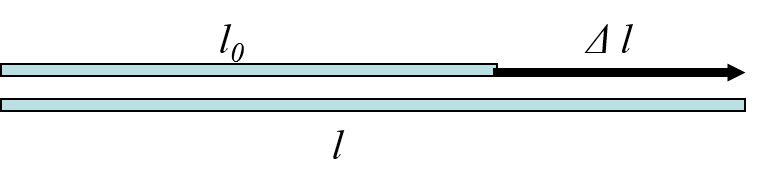
\includegraphics{1d-pretvoreni}
	\caption{Protažení tyče}
	\label{fig:1d-pretvoreni}
\end{figure}

\begin{align}
	E^L &= \frac{1}{2} \frac{l^2 - l_0^2}{l_0^2} = \frac{1}{2} (\lambda^2 - 1)\\
	E^A &= \frac{1}{2} \frac{l^2 - l_0^2}{l^2} = \frac{1}{2} (1 - \lambda^{-2})\\
	\varepsilon &= \frac{l - l_0}{l_0} = \lambda - 1\\
	E^C &= \ln\left(\frac{l}{l_0}\right) = \ln(\lambda)
\end{align}
% Doplnil bych graf v tlaku a řekl které jsou konečné

\tikzsetnextfilename{porovnani-tenzoru-pretvoreni}
\begin{figure}[H]
	\centering
	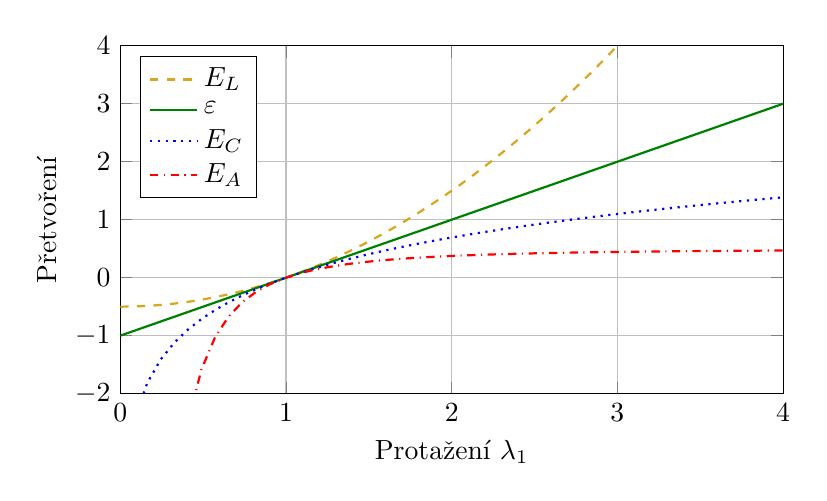
\begin{tikzpicture}
	\begin{axis} [xlabel = {Protažení $\lambda_1$}, ylabel = {Přetvoření},
		grid, height = 6cm, width = 10cm,
		xmin = 0, xmax = 4, ymin = -2, ymax = 4,
		xtick distance = 1, ytick distance = 1,
		legend pos = {north west}, legend cell align={left}]
		\addplot[domain=0:4, samples=50, dashed, thick, Goldenrod] {1/2*(x*x-1)};
		\addplot[domain=0:4, samples=2, solid, thick, Green] {x-1};
		\addplot[domain=0:4, samples=50, dotted, thick, Blue] {ln(x)};
		\addplot[domain=0:4, samples=50, dashdotted, thick, Red] {1/2*(1-1/(x*x)};
		\legend{$E_L$, $\varepsilon$, $E_C$, $E_A$}
	\end{axis}
	\end{tikzpicture}
	\caption{Porovnání tenzorů přetvoření při~jednoosém tahu}
	\label{fig:porovnani-tenzoru-pretvoreni}
\end{figure}
